\documentclass[10pt,twocolumn,letterpaper]{article}

\usepackage{statcourse}
\usepackage{times}
\usepackage{epsfig}
\usepackage{graphicx}
\usepackage{amsmath}
\usepackage{amssymb}

% Include other packages here, before hyperref.

% If you comment hyperref and then uncomment it, you should delete
% egpaper.aux before re-running latex.  (Or just hit 'q' on the first latex
% run, let it finish, and you should be clear).
\usepackage[breaklinks=true,bookmarks=false]{hyperref}


\statcoursefinalcopy


\setcounter{page}{1}
\begin{document}


%%%%%%%%%%%%%%%%%%%%%%%%%%%%%%%%%%%%%%%%%%%%%%%%%%%%%%%%%%%%%%%
% DO NOT EDIT ANYTHING ABOVE THIS LINE
% EXCEPT IF YOU LIKE TO USE ADDITIONAL PACKAGES
%%%%%%%%%%%%%%%%%%%%%%%%%%%%%%%%%%%%%%%%%%%%%%%%%%%%%%%%%%%%%%%



%%%%%%%%% TITLE
\title{Forecasting Airport Waiting Time using Machine Learning Models}

\author{Xintong Li\\
{\tt\small xli2224@wisc.edu}
\and
Yaqi Jie\\
{\tt\small yjie2@wisc.edu}
\and
Jiayi Gao\\
{\tt\small jgao244@wisc.edu}
}

\maketitle
%\thispagestyle{empty}



% MAIN ARTICLE GOES BELOW
%%%%%%%%%%%%%%%%%%%%%%%%%%%%%%%%%%%%%%%%%%%%%%%%%%%%%%%%%%%%%%%


%%%%%%%%% ABSTRACT
\begin{abstract}
   At the airport, due to too many uncontrollable factors in the customs clearance process, it is difficult for passengers who want to catch the next flights to control their time. In this case, the airport needs to control the average waiting time within a reasonable range. It would be better to let passengers know their expected waiting time. This project aim to find a machine learning model that forecast the possible waiting time that takes for passengers to pass the customs. The data set we used is from a HTML table from United States Customs and Border Protection(CBP). After we performed the feature selection, we found the feature importance of the "us\textunderscore citizen" and "non\textunderscore us \textunderscore citizen" were much higher than other features. Thus we discuss the result separately, one put these two features into our estimators and one did not put. Algorithms of k-nearest neighbor, Decision Tree, Random Forest, XGboost, and logistic regression were used to train and test the accuracy. We also used confusion matrix, MaNemar’s test, ROC curve, and F1 score to show the performance of each model. As a result, we found that decision tree is the best option among all the models.
\end{abstract}

%%%%%%%%% BODY TEXT

%-------------------------------------------------
\section{Introduction}
%-------------------------------------------------

With the refinement of the schedules and the combined transportation on a single journey, people appear to be willing to gain more personal control over their waiting time in the airport to pass the customs. However, with the complicated situation and the costly loss of missing a flight, people tend to prepare more waiting time in the airport to avoid these costs. On the other hand, the estimated waiting time under a certain condition is also essential for the airport coordinators to arrange the waiting time more efficiently. 


In October 2021, flight bookings to destinations throughout the United States have reached 70 percent of pre-pandemic levels—52 percent of them were for international inbound flights, according to travel tech provider Travelport. The vast majority of foreign nationals, including those from the 26-nation European Schengen area, the United Kingdom, Ireland, Brazil, China, Iran, and South Africa, who had been restricted from entering the United States since March 2020, will be allowed to enter the United States as long as they provide proof of vaccination.\cite{website} According to the International Air Transport Association (IATA), average passenger processing and wait times have already doubled from what they were during peak travel periods pre-pandemic. As the vaccination policies for U.S. citizens and international travelers are different, a model that could predict the average waiting time of passengers with different citizens would be more helpful for the current situation, and it is important to figure out the different waiting time for U.S. citizens and non-U.S. citizens. Therefore, in additions to the estimators above our alternate model used the us-ave-wait and non-us-avg-wait estimators to predict the influence of having a U.S. citizenship.

In order to provide more information for travelers to help them plan their trip, and for airport coordinators to arrange the customs service, we built our model based on the data of airport wait times of Chicago O’Hare International Airport, which is the closet international airport to University of Wisconsin-Madison, from the U.S. Customs and Border Protection database\cite{CBPwebsite} in the year 2015 to 2021. After eliminating some factors that are unrelated to the average waiting time by their nature, we tested on the feature importance score of the remaining estimators, and we picked the seven with higher scores: us\textunderscore avg\textunderscore wait, non\textunderscore us\textunderscore avg\textunderscore wait, passengers, flights, booths, early morning, early evening.

To find the most accurate classification algorithm to predict the average waiting time of passengers, we tested on Logistic regression, XGBoost, K nearest Neighbours, Decision Tree, and Random Forest. We used 70\% of our data as training data and 30\% for test and computed the training and testing accuracy for each algorithm above. At the end, we used the confusion matrix to evaluate the algorithms.




%-------------------------------------------------
\section{Related Work}
%-------------------------------------------------
The traditional queueing theory discusses problems regarding waiting lines, which includes but is not limited to building queueing models to help people calculate the exact queue waiting time in a mathematical way. Since the queueing theory makes the waiting time for the client accessible, the faculties could better understand the client satisfaction and will make better decisions on their time arrangement. Thus, queueing theory is widely used in Business field as it helps executors to make better business decisions. In this project, we are planning to combine machine learning and queueing theory to explore a real life problem in an airport scenario and attempt to create a prediction model to help people find out the possible time they have to take in the passport checking line.

Previous study of the waiting time prediction in queueing waiting time has been conducted in a machine learning way by Deriaz and Kyritsis in 2018.\cite{waitingtimeprediction} Their targeted population are the the industries that need queues and they evaluated how the machine learning of waiting time prediction could bring benefit to these industries. They applied neural network with 2-hidden layers to fully train the data. Even though their results cannot be used to compare with queueing theory directly, it is a creative way to apply neural network into a classic math problem.
 
Another interesting study conducted by Pak et al discussed the waiting time for patients in an emergency department of a hospital \cite{waitingemergency}. In order to improve the prediction model for the waiting time of ED patients, they applied Ridge, LASSO, as well as OLS regression to fit a linear model. This gives us inspiration on the later regression model that applied in our project. However, unlike Pak's research, which are all numerical variables, we included some binary variables to complete the classification model such as decision tree, 
XGBoost, and random forest.



%-------------------------------------------------
\section{Proposed Method}
%-------------------------------------------------
\subsection{Logistic regression}
Logistic regression is a simple statistical method that widely applied in order to find the probability of the result of a certain event. The result of the event should be binary, for example, yes/no, true/false, and win/lose. In other words the logistic regression performs a logistic function to build models for binary dependent variables. The most commonly used logistic regression model could be written as the following:
$$
\pi_{i} = \frac{exp(\beta_{0}+ \beta_{1}x_{i1}+\cdot+\beta_{ip})}{1+exp(\beta_{0}+ \beta_{1}x_{i1}+\cdot+\beta_{ip})}
$$
Where $\pi_i = x_{i1},x_{i2},......x_{ip}$. Maximum Likelihood estimation will be used in the logistic regression algorithm to find the best coefficient from the training data since the MLE helps reduce the error in the predicted probability in the model. For example, sometimes the best coefficient we gain from the final model might predict a value that very close to our default value 1 (for example, male) or a value very close to 0 (for example, female).  In this case, MLE is applied to avoid those situations. The logistic regression model we will apply in this project is a linear model for binary classification. Another thing to be noticed is that since logistic regression automatically assumes no noise in the dataset, we need to carefully clean our data before using them. 


\subsection{K-Nearest Neighbor}
In general, K-NN classification considers the nearest k neighbors to predict the class for an unknown data point. The nearest neighbors are those data points with the smallest distance from our new data point in the feature space. K is the number of such data points that we consider in the algorithm, which means it is the only hyperparameter we will tune. There are a lot of distance metrics to calculate distance like Euclidean distance, Hamming distance, Manhattan distance, and Minkowski distance. In this project, we will only use Euclidean distance to find the nearest neighbors. The function below shows how to calculate the distance in n-dimensional Euclidean space. P and q are two points in Euclidean n-space. $q_i$ and $p_i$ are Euclidean vectors, starting from the origin of the space.The formula is as the following:
$$
d(p,q) = \sqrt{\sum^n_{i=1} (q_{i)-p_{i})^2}}
$$

For each coming new data point, we use all the points in the training set and find new data point’s ‘K’ Nearest Neighbors. 


\subsection{Decision Tree}
The goal of using decision trees is to create a training model that can predict the class label of the target variable by learning simple decision rules inferred from the training data set. The decision tree classifies the examples by sorting the examples from the root of the tree to a certain leaf node, and the leaf node provides the classification of the example. There are some assumptions we need to make before using the decision tree. The whole training set should be considered as the root. The feature value is preferably classified. Records are distributed recursively based on attribute values. We use statistical methods for ordering attributes as root nodes or internal nodes\cite{ML}. In this project, we used Entropy or Gini Impurity to grow the decision tree. Entropy is a measure of the randomness of the information being processed. The higher the entropy, the harder it is to draw any conclusions from this information. Gini Impurity was also used to evaluate splits in the dataset.  Information gain measures how well a given attribute separates training examples according to its target classification. The function below defines the criterion that maximized information gain and minimized entropy.
$$
\text{GAIN} (D,x_{j}) = H(D) - \sum_{v \in \textit{values}_{x_{j}}} \frac{\lvert D_{v} \rvert }{D} H(D_{v})
$$
D is the training set at the parent node, and $D_v$ is a dataset at a child node upon splitting.
\subsection{Random Forest}
Random Forest method combines the output of multiple decision trees to reach a single result.  For classification tasks, the output of the random forest is the class selected by most trees. The key difference between decision trees and random forests is that random forest generates a random subset of features, which ensures low correlation among decision trees. While decision trees consider all the possible feature splits, random forests only select a subset of those features. Random forest corrects the habit of decision tree overfitting the training set\cite{Hastie2008}.

\subsection{XGBoost}
As an ensemble technique in machine learning, boosting helps improve our models by adding new models into existed models repeatedly to re-weight the training data and  correct the possible errors until no improvement can be made. Gradient boosting method predicts the residuals of previous models and forms the prediction into new models, then adds the new models together to create the final model. And as one of the implementations of Gradient boosting, the XGBoosting does the jobs in a faster and more optimized way compared to other implementations of Gradient Boosting. 

\subsection{ K-fold Cross-Validation}
Cross-validation is used to estimate the performance of a machine learning model on unseen dataset. K-fold cross-validation is a special case of cross-validation where we iterate over a dataset k times. In each iteration, the data set is split into k parts: one part is used for the validation data set, and the remaining k-1 parts are combined into a training subset for model evaluation.\cite{note} We can calculate the cross-validation performance as the arithmetic mean of k performance estimates from the validation data set. This method ensures that all samples are used and prevents overlap.

%-------------------------------------------------
\section{Experiments}
%-------------------------------------------------


\subsection{Data set}
United States Customs and Border Protection (CBP) is a federal agency tasked with the responsibility of protecting the nation’s borders from a variety of threats.\cite{CBP} The raw dataset we will be applied in our project originated from the CBP’s website, \url{https://awt.cbp.gov/}. As stated in our motivation, we are interested in the prediction of the average waiting time for each passenger in the Ohare international airport in the last 7 years. According to the data dictionary provided by CBP, the waiting time is defined as the time it takes for each passenger to clear the passport control area. In this case, we extracted the records for the ORD from 2015 to 2021 and converted the records from the HTML table into a single CSV file. Furthermore, since the headers for each column in the raw dataset were too concise to understand, we renamed the column headers according to the meaning of the variable. Our final raw dataset contains 44053 observations and 20 features in total.  

\begin{figure}[h]
\centering
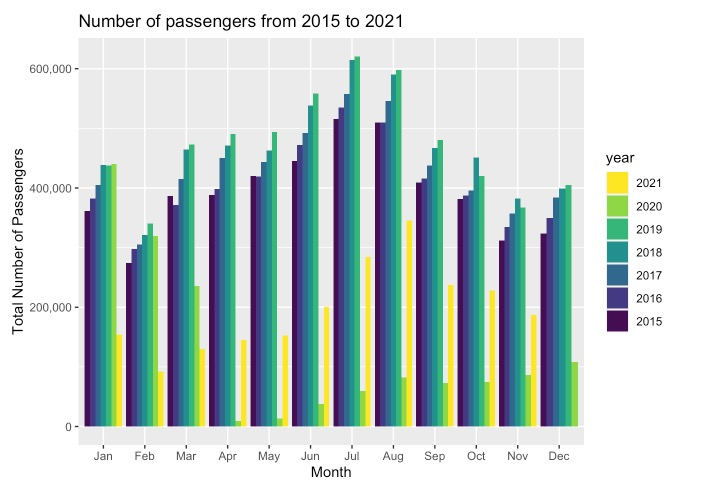
\includegraphics[scale=0.35]{figures/Dataset.jpeg}
\caption{Total number of passengers each month from 2015 - 2021}
\end{figure}
Figure 1 provides us a general look of the number of passengers each month from 2015 to 2021. One thing to be noticed is that during 2020, which is the pandemic period, there was a obvious decrease in the number of passengers. As we discussed in the introduction, the possible reason for this dramatic decrease of the number of passengers might due to the reduction of the number of flights.

\subsection{Data processing}
\subsubsection{Processing}

Since the data were provided by the U.S government, the dataset was already complete and cleaned. In this case, no data cleaning were needed. However, we collected information online for possible variables that may have influences on the average waiting time. Some of the variables have already existed in the dataset such as the number of passengers on that day. We also created new columns based on the existed variables in the dataset. More specifically, we added the “weekend” column to our cleaned dataset by checking the date of the flight. This is a binary variable with the value 1 standing for Saturday or Sunday, and the default value, 0, standing for the weekdays. Another column that has been added to our dataset was the “time of day”. This column tells us what time period of the day was the recorded flight. The variable contains 6 categories. To put in detail, the “overnight” is from 1 am to 5 am; “early morning” is from 5 am to 8 am; “morning” is from 8 am to noon; “afternoon” is from noon to 5 pm; “early evening” is from 5 pm to 8 pm; and “late evening” is from 8 pm to 1 am. In addition, to make it easier for us to classify the features, we also created 6 new columns based on the “time of day” feature with each observed flight’s specific time of day being value 1, and others remaining as the default value, 0.

After many web-based searches, we conclude that the ideal waiting time for the majority of the passengers from disembarking to the end of the border crossing is around 25 minutes. However, the information recorded on the CBP website only includes the waiting time for each passenger in line for the passport checking. Thus, we narrowed the boundary of our average waiting time down to 15 minutes. And a new feature called “avg wait time” is created with label 1 as the waiting time is greater than15 and 0 otherwise.

\subsubsection{feature selection}

Before we calculate the feature importance, we exclude some variables from the processed dataset since these variables seem to have little relationship with the average waiting time such as maximum waiting time for each passenger. In this case, 12 variables remained in our dataset. However, there might be noises included in these 12 variables and we cannot make sure that all of these 12 variables will make contributions in model building. Hence, we calculated feature importance toward the output variable using the Extra Tree Classifier function and only selected variables that have a great influence on airport waiting time as our estimator to find the models. After considering the feature importance, we decided to use 7 features as our input for modeling, early evening, early morning, flights, booths, passengers, us\textunderscore citizens, and non\textunderscore us\textunderscore citizens. 

\subsection{Model Training}
After processing and feature selection, we divided the whole dataset into 70\% of training data and 30\% of testing data using train\textunderscore test\textunderscore split method in sklearn. For each method we analyzed in the previous section, we created two models accordingly. On model used all 7 features we selected from feature selection, and the other one used features other than us\textunderscore citizens and non\textunderscore us\textunderscore citizens. We used GridSearchCV to tune the hypermeter and record the best parameter. K\textunderscore fold Cross\textunderscore validation can be utilized to evaluated our model best estimator. We calculated the average cross\textunderscore validation score for each model.

\subsubsection{Logistic Regression}
We applied \textit{LogisticRegression} function in the sklearn.linear\textunderscore model package to create our logistic regression model. The hyper parameter, c, we chose are from 0.001 to 100 with a step factor 10. The following formula calculates the mean squared error of the model. The smaller MSE we have, the more accurate the model will be. 
\begin{center}
$MSE = \frac{1}{n} \sum_{i=1}^{n}(Y_{i} - \hat{Y_{i}})^2$
\end{center}


\subsubsection{ K nearest neighbor}
We used KNeighborsClassifier from sklearn to train the model. Since features are in different scales, we assembled KNeighborsClassifier and StandardScaler together to create a pipeline. N-neighbours is the only hyperparameter we tuned. We first loop over K from 1 to 100, and then narrow it down to 60. At last, we used GridSearchCV to find the best hyperparameter and recorded the accuracy of this best estimator on the test model. 

\subsubsection{decision tree}
There are two parameters we tuned in DecisionTreeClassifier: max\textunderscore depth and criterion. We first loop over max\textunderscore depth from 1 to 100 to find out changes in test accuracy. Then, we narrow this hyperparameter down to 20 with a step of 1. In order to select the best parameters, we use GridSearchCV to generate candidates from a grid of parameter values specified by the param\textunderscore grid parameter. One grid is max\textunderscore depth from 1 to 16 with a step of 1, the other one is criterion values in ['gini', 'entropy']. Finally, we record the accuracy of the best estimator on the test model.

\subsubsection{Random Forest}
There are three parameters we tuned in DecisionTreeClassifier: max\textunderscore depth, n\textunderscore estimators, and criterion. Similar to Decision Tree, we use GridSearchCV to generate candidates from a grid of parameter values specified by the param\textunderscore grid parameter. The first grid is criterion values in ['gini', 'entropy'], the second one is max\textunderscore depth values in [1, 10, 50, 100, 150], and the last one is n\textunderscore estimators values in [10, 20, 50, 100, 150]. We calculated the mean of K-fold cross-validation score of the best estimator and record the accuracy on the test model.

\subsubsection{XGBoost}
Similar to the Decision tree, two hyperparameters that we tune in XGboost are max\textunderscore depth and learning\textunderscore rate. We first loop over max\textunderscore depth from 1 to 50. After checking test set accuracy, we narrow max\textunderscore depth down to 20. The parameter values specific for max-depth are [1,2,3,....20], while values specific for learning\textunderscore rate are [0.1, 0.01]. We use the best estimator from GridSearchCV and record its accuracy on the test model.


\subsection{Software}

We use excel to hold our dataset, R studio for data processing, Jupyter Notebook for modeling and graphing. 

\subsection{Hardware}

The hard wares that support our project is each group member's own laptop.

%-------------------------------------------------
\section{Results and Discussion}
%-------------------------------------------------

Before entering the detail result of our methods, there is one thing to be noticed in order to fully understand the following discussion. We trained our model for two different situations, one with the features “us\textunderscore citizens” and “non\textunderscore us\textunderscore citizen”, and the other one without these two features. The reason we have these two different situation is that these two features display high feature importance in our feature selection part. According to the feature importance diagram below (Figure 2.),  the importance of "US" and "non\textunderscore US" are way above other features. It makes sense if we explain this by our real-world experiences. It might take on us citizens passengers longer to pass the booth as the customs need to check the passports and ask questions. To avoid domination of these two features among all features, we separated our discussion into two situations. 
\begin{figure}[h]
\centering
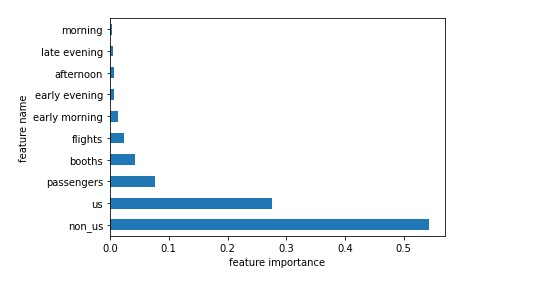
\includegraphics[scale=0.5]{figures/feature importance.jpg}
\caption{Feature Importance}
\end{figure}
The following two tables are brief summaries of our test ac curacies for the two situations we mentioned above. As we expected, the test accuracy for models with "us\textunderscore citizens” and “non\textunderscore us\textunderscore citizens” are all around 96\%, which are much higher than the test accuracy for models without these two features (around 70\%).  

Table 1 is a summary of the results obtained from each model with residency in estimators. 
	\begin{table}[h!]
		\begin{tabular}{|c|c|c|}
			\hline
			Model & Hyperparameter & Accuracy\\
			\hline 
			\hline
			Logistic regression & c=0.01 & 95.26\%\\
			\hline
			\multirow{XGBoost}  & \small{max\_depth = 5} & \multirow{96.97\%}\\
			& \small{learning\_rate= 0.1} & \\
			\hline
			KNN  & k = 21 & 96.45\%\\
			\hline
			\multirow{Decision Tree}  & \small{max\_depth = 6} & \multirow{96.61\%}\\
			& \small{criterion = ‘gini’} & \\
			\hline
			\multirow{Random Forest} & \small{max\_depth = 10} & \multirow{96.97\%}\\
			& \small{criterion = ‘gini’}& \\
			& \small{n\_estimators= 50}& \\
			
			\hline		
		\end{tabular}\\
		\caption{Best Hyperparameters and Test Accuracy for each Method (residency included)}\label{results}
	\end{table}

Table 2 is a summary of the results obtained from each model without residency in estimators. 
	\begin{table}[h!]
		\begin{tabular}{|c|c|c|}
			\hline
			Model & Hyperparameter & Accuracy\\
			\hline 
			\hline
			Logistic regression & c=1 & 69.78\%\\
			\hline
			\multirow{XGBoost}  & \small{max\_depth = 5} & \multirow{70.39\%}\\
			& \small{learning\_rate= 0.1} & \\
			\hline
			KNN  & k = 55 & 69.59\%\\
			\hline
			\multirow{Decision Tree}  & \small{max\_depth = 5} & \multirow{69.95\%}\\
			& \small{criterion = ‘gini’} & \\
			\hline
			\multirow{Random Forest} & \small{max\_depth = 10} & \multirow{70.31\%}\\
			& \small{criterion = ‘entropy’}& \\
			& \small{n\_estimators= 100}& \\
			\hline
		
		\end{tabular}\\
		\caption{Best Hyperparameters and Test Accuracy for each Method (residency excluded)}\label{results}
	\end{table}


\subsection{Logistic Regression}
The test accuracy for logistic regression model with features "us\textunderscore citizen" and "non\textunderscore us\textunderscore citizen" are 95.26\% and for the model without these two features is 69.78\%. In the model with the "us\textunderscore citizen" and "non\textunderscore us\textunderscore citizen", the best hyperparameter we  found is 0.001, but in the model without these two features, the best hyperparameter we found is 1. Furthermore, the experiment with residency has the MSE of 0.04 while the experiment without residency has MSE of 0.30. We also created an ROC curve, and Figure 3 shows the performance of the two cases. From this figure, we can see how well the model performs when using features "us\textunderscore citizen" and "non\textunderscore us\textunderscore citizen"

\begin{figure}[h]
\centering
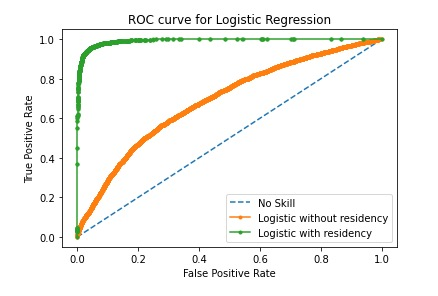
\includegraphics[scale=0.55]{figures/LR.jpeg}
\caption{ROC curve for Logistic Regression with residency (AUC : 0.992) vs without residency (AUC : 0.691)}
\end{figure}

\subsection{K nearest neighbor}
KNN method achieves its best accuracy 96.45\% in the experiment containing residency at k = 21, which is the second lowest accuracy among all method. It achieves its best accuracy 69.59\% in the experiment without residency at k = 55, which is the lowest accuracy among all method. Figure 4 and Figure 5 show the performance changes of the KNN model when we tune the parameter n\textunderscore neighbour in two cases. These two graphs are in line with our expectations. We prevented overfitting as k increased, so training accuracy decreased, and test accuracy increased. It is as expected that KNN results lower accuracy scores because this method is a little simple compared with other methods. It only contains one parameter and has a limited capability of adjusting the model according to the data. The accuracy score could possibly be improved with other k values, but it is not worth it to try many different k values as this method is expected to have low accuracy score because the structure of its algorithm. 

\begin{figure}[h]
\centering
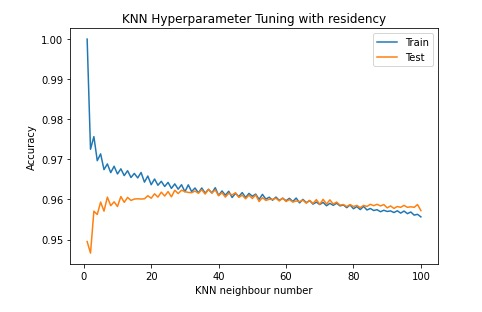
\includegraphics[scale=0.48]{figures/KNN with Residency.jpeg}
\caption{KNN hyperparameter tuning with residency}
\end{figure}

\begin{figure}[h]
\centering
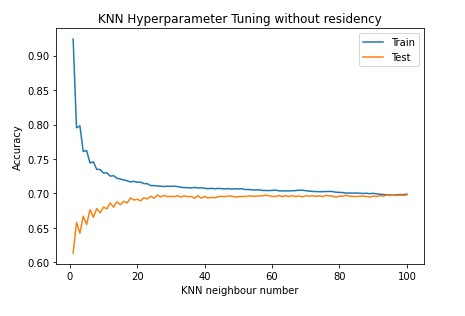
\includegraphics[scale=0.5]{figures/KNN without residency.jpeg}
\caption{KNN hyperparameter tuning without residency}
\end{figure}


\subsection{Decision Tree \& Random Forest \& XGBoost}

Decision tree, Random Forest and XGboost models achieve 96.61\%, 96.97\%, and 96.97\% accuracy respectively in the experiment containing residency while these models achieve test accuracy of 69.95\%, 70.31\%, and 70.39\% respectively in the experiment without residency. This result is reasonable because the identity of the passenger has a great influence on the waiting time. If we include us\textunderscore wait\textunderscore time and non\textunderscore us\textunderscore wait\textunderscore time in X, their variation largely determines the changes in the label, so we get a high degree of accuracy. The accuracy we got from these three models is similar. Test accuracy generated from the Decision Tree is only a little lower than the other two models. We also used K-fold cross-validation to do the model evaluation and got analogous results as GridSearchCV. Since we got high accuracy in the experiment containing residency, we only do further research in the case without residency. The Decision Tree macro average F1 score is 0.57, and the Random Forest and XGBoost macro average F1 scores are 0.60 and 0.61 respectively. We also created a precision recall curve in order to test the performance of these three model. The three lines shown in Figure 6 essentially coincide, so we can conclude that the accuracy of these three models is basically the same.

\begin{figure}[h]
\centering
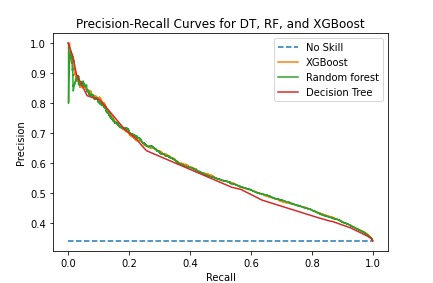
\includegraphics[scale=0.57]{figures/Recall.jpeg}
\caption{Precision-Recall Curves for Decision Tree, Random Forest, and XGBoost}
\end{figure}

Due to the similar performance, we want to understand if the Random Forest model is the same as the XGBoost model. Therefore, we did a MaNemar’s test on these two models. The confusion matrix is shown in figure 7. We got a p\textunderscore value 8.372e-09 after running McNemar’s test over two models’ predictions. Because p\textunderscore value is less than 0.05, we reject the null hypothesis which states that the two models are the same. Finally, we conclude that there are significant differences between the two models.

\begin{figure}[h]
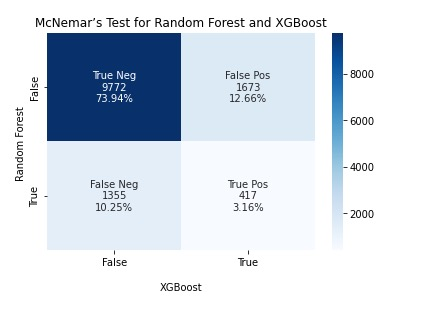
\includegraphics[scale=0.58]{figures/McNemar's test.jpeg}
\caption{McNemar's test of Random Forest and XGBoost}
\end{figure}

\subsection{Discussion}
Based on the results discussed above (table 1. and table 2.), the logistic regression and KNN performs lower accuracy scores for both cases with or without taking residency into consideration. The accuracy scores for decision tree, random forest, and XGBoost methods are similar in both cases. Therefore, we would recommend the later researchers to consider using decision tree model for similar studies. Another reason we recommend decision tree over random forest and XGBoost is that with similar result, the random forest and XGBoost methods require more cost and time. Another interesting thing needs to be mentioned in our result is that the residency dominates in our machine learning process. We think a possible reason behind it is that the average waiting time equals the weighted average of the average waiting time of U.S and non-U.S. residences.

There are few limitations in our model need to be noticed. First, the average waiting time in the raw data set was a continuous variable, but we converted it to classification to reduce the complexity of our model and to enhance the accuracy. In this case, converting the feature from continuous into binary might abandoned some useful information for modeling. It might also be one reason that the accuracy scores of Decision Tree, Random Forest, and XGBoost are similar. Another limitation is that the average waiting time in the airport customs could be significantly influenced by the COVID-19, which increase the uncertainty, but we did not compute the average waiting time before and after the COVID-19 situation separately.


%-------------------------------------------------
\section{Conclusions}
%-------------------------------------------------
In this project, our goal is to find the most fit machine learning model that can accurately predict the average customs waiting time given some characteristic conditions. We examined several potential models, trained them with hyperparameter tuning, and evaluated the performance of each model in terms of accuracy, confusion matrix, and F1 score. As we analyzed in the previous section, since the identity of the passenger has a decisive influence on the waiting time for customs clearance, we trained the models in two situations. 

According to table 1 and table 2 above, the models that with the highest test accuracy in the experiment with residency are the random forest and XGBoost, which both have the test accuracy of 96.97\%. And the models that have the highest test accuracy in the experiment without residency is the XGboost with test accuracy of 70.39\%. However, the accuracy we get through the decision tree is only about 0.5\% lower than the best-performing model in both cases. Compared with Random Forest and XGBoost, the decision tree is relatively simple to perform and is less time-consuming, so we suggest using Decision Tree to make predictions. 

According to the result we above, we can provide some insights to the ORD airport. Our results show that the numbers of US citizens and non-US citizens have a decisive influence on waiting time. Since the identity of passengers cannot be changed, the airport can reasonably control the average waiting time by adjusting the number of booths and air crafts. At the same time, we recommend the airport to predict the average waiting time based on our model and display the corresponding feature information and prediction results on the official website. Many passengers may go to other cities immediately after they got off an international flight, so estimating the waiting time in advance can prevent them from missing the flight due to a long waiting time.

In this future work, we plan to focus on the research for the pandemic period and use the possible model to predict the average waiting time under the post pandemic situation. Advanced techniques such as deep learning or LASSO regression might be applied in the future work to find a better performed model. 

%-------------------------------------------------
\section{Contributions}
%-------------------------------------------------
Our group has three people, Xingtong, Yaqi, and Jiayi. In this project, we first discussed how to clean and merge the data set together. We then separated the data set into the training set and test set collaboratively. 

For the computation part, We built models and make decisions on the model selection part collaboratively. More specifically, we discussed the feature selection together and Xingtong performed the coding part for the feature importance graph. For the modeling part, Jiayi did the logistic regression, Xingtong did K-nearest neighbor, decision tree, xgboost, and Yaqi did the random forest. And we all went over the visualization part together and made decision on the graph selection together.

For the writing part of this project, Yaqi wrote the introduction; random forest in the proposed method;Random Forest in the experiment; K-nearest neighbor in the result; and part of the discussion and conclusion. Jiayi wrote the abstract; related work; logistic regression and XGboost in the proposed method; Data set, Data processing, and feature selection in the experiments; Introduction and logistic regression in the result and discussion; as well as part of the conclusion. Xingtong wrote K-nearest neighbor, decision tree,and K-fold Cross-Validation in the proposed method; model training, k-nearest neighbor, decision tree, random forest, and xgboost in the experiment; decision tree & random forest & XGBoost and part of discussion in the result and discussion; and also apart of the conclusion.

Though we had different tasks in this project, we helped each other while any of us are running into problems.


%-------------------------------------------------
\section{Code}
%-------------------------------------------------

The code and plot for this project can be accessd at the following Github link: \url{https://github.com/Kaylee0501/451_project}

{\small
\bibliographystyle{ieee.bst}
\bibliography{bibliography.bib}
}



\end{document}
